\documentclass[
%===============================================================
%	DOCUMENT PREFERENCES
%===============================================================
	parskip		=	half,			% remove first-row indent in new paragraph
	headheight	= 	12pt,			% header height
	footheight 	= 	16pt,			% footer height
	headsepline,						% header separator line
	footsepline,						% footer separator line
	abstracton,						% Abstract headers
	headinclude	=	false,		
	footinclude	=	false,
	listof		=	totoc,			% List of ... in TOC
	toc			=	bibliography,	% Bibliography in TOC
	draft		=	false
]{scrreprt}


% Language and general symbol preferences
\usepackage[ngerman, english]{babel}
\usepackage[utf8]{inputenc}
\usepackage{soul}					% hyphening, etc.
\usepackage[super]{nth}				% superscript "n-th" (counting, etc.)
\usepackage{enumitem}

% Page preferences
\usepackage[a4paper]{geometry}				
\geometry{
	a4paper,
	margin		=	2.5cm,
	left		=	3.3cm,
	foot 		= 	1.0cm
}

% Font preferences
\usepackage{couriers}
\KOMAoptions{fontsize=12pt}			% 12pt font size
\addtokomafont{disposition}			% Serif font for chapter headings
	{\rmfamily\bfseries}

\usepackage{setspace}				% 1.5x line spacing	
\onehalfspacing

% Header & Footer preferences
\usepackage{scrlayer-scrpage}		% Clear default settings
\pagestyle{scrheadings}
\clearpairofpagestyles

\ihead{Studienarbeit (T3101)}	    % Header left	(Type)
\automark{chapter}					% Header right	(Chapter)
\ohead{\rightmark}
\ifoot{DHBW Stuttgart}				% Footer left	(School)
\cfoot{Goldschmidt, Rudzinski}		% Footer center	(Author)
\ofoot[\pagemark]{\pagemark}			% Footer right	(Page mark)

%===============================================================
%	ADDITIONAL PREFERENCES
%===============================================================

% Bibliography preferences
\usepackage[style=ieee]{biblatex}
\bibliography{studienarbeit_pwa.bib}

% Management packages
\usepackage[titles]{tocloft}			% ToC management
\setlength{\cftbeforechapskip}{5pt}
\usepackage{array}					% Table management
\usepackage{multirow}
\usepackage{acronym}					% Acronym management
\usepackage{graphicx}				% Figure management
\usepackage{subfig}
\usepackage{hyperref}				% Referencing management
\hypersetup{}
\usepackage{minted}					% Source code management
\setminted[sql]{
	autogobble,
	baselinestretch=1,
	breaklines,
	frame=lines,
	fontsize=\footnotesize,
	framesep=3mm
}
\setminted[json]{
	autogobble,
	baselinestretch=1,
	breaklines,
	frame=lines,
	fontsize=\footnotesize,
	framesep=3mm,
	linenos
}
\setminted[xml]{
	autogobble,
	baselinestretch=1,
	breaklines,
	frame=lines,
	fontsize=\footnotesize,
	framesep=3mm,
	linenos
}

\setminted[text]{
	autogobble,
	baselinestretch=1,
	breaklines,
	frame=lines,
	fontsize=\footnotesize,
	framesep=3mm,
	linenos
}

\setminted[TypeScript]{
	autogobble,
	baselinestretch=1,
	breaklines,
	frame=lines,
	fontsize=\footnotesize,
	framesep=3mm,
	linenos
}

\setminted[Swift]{
	autogobble,
	baselinestretch=1,
	breaklines,
	frame=lines,
	fontsize=\footnotesize,
	framesep=3mm,
	linenos
}

\usemintedstyle{manni}	
\usepackage[T1]{fontenc}
\usepackage{inconsolata}			
	
% Misc
\setcounter{tocdepth}{1}				% Remove sub-sections from TOC
\setcounter{lofdepth}{2}
		% to make images being floatable by text
\usepackage{float} 			
\usepackage{wrapfig}

\usepackage{standalone}                       % to include spider diagrams

\usepackage{tabularx} % for breaking table entries
\newcolumntype{C}{>{\centering\arraybackslash}X} % centered "X" column

%===============================================================
%	CUSTOM COMMANDS
%===============================================================

% Title page image handling
\newcommand*{\vcenteredhbox}[1]{
	\begingroup
	\setbox0=\hbox{#1}\parbox{\wd0}{\box0}
	\endgroup
}

% Remove page break on abstract
\newenvironment{absolutelynopagebreak}
{\par\nobreak\vfil\penalty0\vfilneg\vtop\bgroup}{\par\xdef\tpd{\the\prevdepth}\egroup\prevdepth=\tpd}

% to use colored circles to show hex color
\usepackage{pict2e}  % to allow any radius
\usepackage[table,usenames,dvipsnames]{xcolor}% http://ctan.org/pkg/xcolor

% Listing package for source code
\renewcommand{\listingscaption}{Quellcode-Ausschnitt}
\renewcommand{\listoflistingscaption}{Quellcodeverzeichnis}

% tables
\usepackage{tcolorbox}
\usepackage{array}
\usepackage{colortbl}
\tcbuselibrary{skins}
\tcbset{tab2/.style={enhanced,fonttitle=\bfseries,fontupper=\normalsize\sffamily,
		colback=yellow!10!white,colframe=red!50!black,colbacktitle=Salmon!40!white,
		coltitle=black,center title}}
	
% Kaviat Diagram
%\usepackage[utf8]{inputenc}
%\usepackage[upright]{fourier}
\usepackage{tkz-kiviat,numprint,fullpage} 
\usepackage{pgfplotstable} 
\usetikzlibrary{arrows}

%===========================================================================

\title{Gegenüberstellung der Entwicklung\\nativer Mobilanwendungen und\\Progressive Web Apps (PWAs)} 
\author{Stefan Goldschmidt\\Oliver Rudzinski}
\date{08. Juni 2020}

%===========================================================================

\begin{document}
\makeatletter
\selectlanguage{ngerman}

%===========================================================================
%	FRONT MATTER
%===========================================================================

	\clearpage
	\hfill
\vcenteredhbox{
\includegraphics[height=2.5cm]{img/logo_dhbw.png}}

\vfill\vfill

\begin{center}
	\rule{\linewidth}{1pt}
	{
		\Huge \bfseries
			\@title
		\par	
	}
	\vspace{-0.2cm}
	\rule{\linewidth}{1pt}
	

	Studienarbeit (T3101)
	\vfill
	
	für den Studiengang \\ \textbf{Informatik}
	
	an der \\ \textbf{Dualen Hochschule \\Baden-Württemberg\\Stuttgart}
	\vfill
	von \\ \textbf{\textsc{\@author}}
\end{center}

\vfill\vfill

\begin{tabbing}
	mmmmmmmmmmmmmmmmmmmmmmmmmm				\= \kill
	\textbf{Abgabedatum} \> \@date \\
	\textbf{Matrikelnummern} \> \texttt{9760520} (Goldschmidt)\\
	\> \texttt{5481330} (Rudzinski) \\
	\textbf{Kurs}	\> TINF17A \\
	\textbf{Hochschulbetreuer} \> Arne Heimeshoff \\ 
	\textbf{Hochschulverantwoftlicher} \> Prof. Dr. Zoltán Zomotor \\
	\textbf{Studiengangsleitung} \> Prof. Dr. Dirk Reichardt \\
	\> Prof. Dr. Carmen Winter
\end{tabbing}
	\thispagestyle{empty}
	
	\pagenumbering{roman}
	
	\clearpage
	\chapter*{Erklärung}
		\vfill
Wir versichern hiermit, dass wir unsere Studienarbeit mit dem Thema:
\begin{center}
	\vspace{1.0cm}
	\textit{\@title}
	\vspace{1.0cm}
\end{center}
selbstständig verfasst und
keine anderen als die angegebenen Quellen und Hilfsmittel benutzt haben. \\


\vfill

\rule{3,5cm}{0.4pt}, \rule{3,5cm}{0.4pt} \hspace{0.38cm} \rule{7cm}{0.4pt}\\
Ort
\hspace{2.9cm}
Datum
\hspace{2.6cm}
Unterschrift \textbf{Stefan Goldschmidt}

\vspace{1cm}

\rule{3,5cm}{0.4pt}, \rule{3,5cm}{0.4pt} \hspace{0.38cm} \rule{7cm}{0.4pt}\\
Ort
\hspace{2.9cm}
Datum
\hspace{2.6cm}
Unterschrift \textbf{Oliver Rudzinski}
	\thispagestyle{empty}
	
	\clearpage
	\begin{abstract}
    
\end{abstract}
		\addtocontents{toc}{\protect\thispagestyle{empty}}
	\thispagestyle{empty}
	
	{\small\tableofcontents}
	\thispagestyle{empty}
	
	\chapter*{Abkürzungsverzeichnis}
		\begin{acronym}[MMMMMM]
 
 	\acro{api}[API]{Application Programming Interface}
	\acro{cli}[CLI]{Command Line Interface}
	\acro{crud}[CRUD]{Create, Read, Update und Delete}
	\acro{css}[CSS]{Cascading Style Sheets}
	\acro{csv}[CSV]{Comma-separated Values}
	\acro{html}[HTML]{Hypertext Markup Langauge}
	\acro{https}[HTTPS]{Hypertext Transfer Protocol Secure}
	\acro{ide}[IDE]{Integrated Development Environment}
	\acro{json}[JSON]{JavaScript Object Notation}
	\acro{mvc}[MVC]{Model-View-Controller}
	\acro{os}[OS]{Operating System}
	\acro{pwa}[PWA]{Progressive Web App}
	\acro{rest}[REST]{Representational State Transfer}
	\acro{scss}[SCSS]{Sassy \acs{css}}
	\acro{ssl}[SSL]{Secure Sockets Layer}
	\acro{ui}[UI]{User Interface}
	\acro{url}[URL]{Uniform Resource Locator}
	\acro{xml}[XML]{Extensible Markup Language}

\end{acronym}

		\addcontentsline{toc}{chapter}{Abkürzungsverzeichnis}
	
	\listoffigures

	\listoftables

	\listoflistings

%===========================================================================
%	MAIN MATTER
%===========================================================================

	\chapter{Einleitung}
		\pagenumbering{arabic}
		\label{chap:einleitung}
		%===========================================================================
%	Einleitung
%===========================================================================
\section{Marktüberblick}

Marktanteile / Nutzung von Mobilgeräten

Für das Jahr 2020 wird erwartet, dass 45\% der Weltbevölkerung ein Smartphone nutzt.
% https://www.statista.com/statistics/330695/number-of-smartphone-users-worldwide/
\cite{StatistaSmartphonesWorldwide}
%https://www.statista.com/statistics/262875/development-of-the-world-population/
\cite{StatistaWorldPopulation}
% 3,5 / 7,79 Milliarden = 45%
Sowohl Unternehmen, die ihre Produkte überwiegend offline vertreiben, als auch die führenden IT-Unternehmen wissen um diesen Trend, denn App-Nutzer sind (potenzielle) Kunden. Auch die Medienbranche verdient mit App-Nutzern Geld, da mit jedem Nutzer ihrer Website oder App die Werbeeinnahmen steigen. 
Newsportale wie Focus Online, BILD, Welt.de oder Spiegel Online gehören 2019 zu den verbreitetsten mobilen Webseiten \cite{StatistaMobileWebsiteNetReach2019}. Diese  Webseiten sind bereits für Mobilegeräte optimiert. Für Entwickler liegt es nahe, die Webseite in einer Mobilanwendung einzubetten, anstatt alle Features in einer nativen Anwendung neu zu entwickeln. Der Nutzer kann diese Anwendungen über einen App Marktplatz beziehen. Mit Bannern und Links versuchen Unternehmen auf ihre Mobilanwendungen aufmerksam zu machen.
Mit dem Konzept der \ac{pwa} könnte dieser Schritt bald obsolet werden, wenn Nutzer nicht mehr eine plattformabhängige App, sondern vielmehr die Webseite selbst als ``Anwendung'' installieren. Bezieht man die vergleichsweise hohen Entwicklungskosten mobiler Anwendungen in diese Rechnung mit ein, besteht eine große Chance, dass die Erweiterung der bestehenden Webseite zur PWA schneller, wartungärmer und insgesamt günstiger ist.

Die Progressive Web App verspricht nicht nur einen einfachen Container um eine Website, sondern auch Offline-Funktionalität, vergleichsweise einfache Entwicklung mit JavaScript und Unabhängigkeit der Plattform. Damit löst sie viele bekannte Probleme einfacher Container Apps um eine Webseite. Nicht selten wird dort die Geduld der Nutzer herausgefordert, da alle Inhalte (Scripte, Stylesheets, Schriftarten, HTML etc.) ständig über eine möglicherweise langsame Datenverbindung heruntergeladen werden müssen.

Der Hohe Marktanteil (60\% in 2019) des mobilen Browsers Google Chrome (welcher die Installation von PWAs voll unterstützt \cite[S. 8]{BeginningPWA}) und Apples Safari für iOS (20\% in 2019), welcher die Unterstützung der PWA stetig erweitert, inspirieren diese Arbeit, die Möglichkeiten der PWA im Vergleich zur nativen App ausführlich zu vergleichen.
\cite{StatistaMobileBrowserMarketShare}

% Mobile shopping app user acquisition costs
%https://www.statista.com/statistics/911981/mobile-shopping-apps-user-acquisition-costs-by-type-gender/

% median cost of app dev in regions by $ per hour$
%https://www.statista.com/statistics/628636/worldwide-mobile-app-development-costs-by-region-by-platform/

% median cost of app dev per hour
%https://www.statista.com/statistics/647807/north-america-mobile-app-development-costs/

% market share mobile browsers
%https://www.statista.com/statistics/263517/market-share-held-by-mobile-internet-browsers-worldwide/

% Leading mobile websites ranked by net reach in Germany
%https://www.statista.com/statistics/425372/mobile-websites-by-net-reach-germany/


%\begin{figure}[h]
%        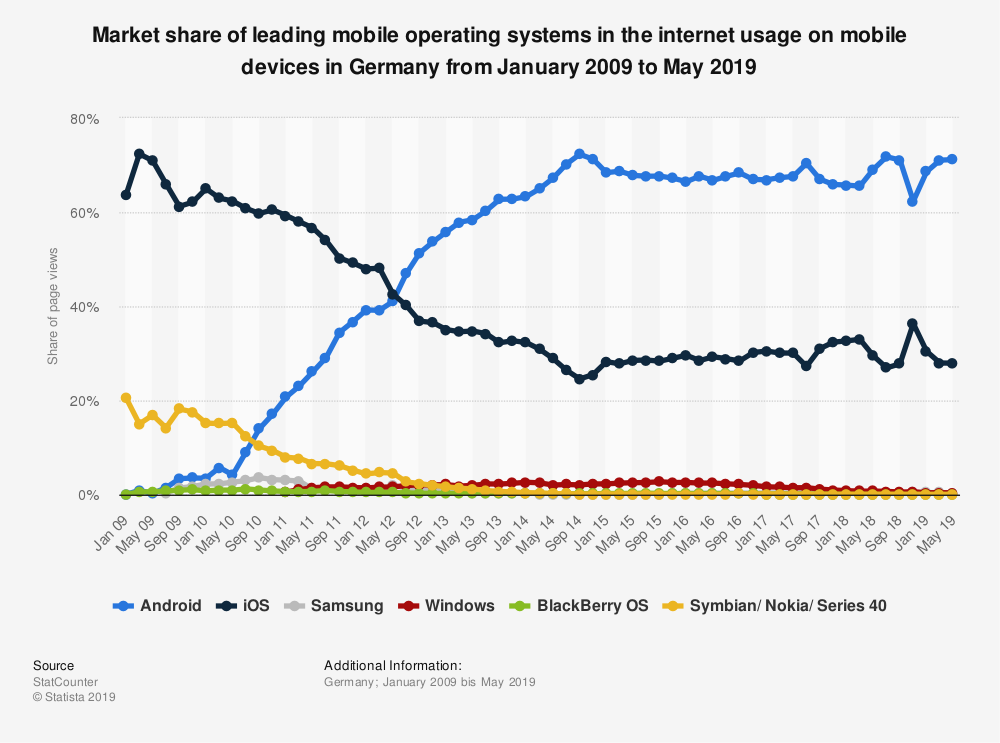
\includegraphics[width=\linewidth]{img/statistic_id461981_market-share-of-operating-systems-in-mobile-internet-usage-in-germany-2009-2019.png}
%        \centering
%        \caption{Market share \cite{StatistaMarketShareSmartphone}}
%        \label{fig:marketshare}
%\end{figure}

%===========================================================================
%	Motivation
%===========================================================================
\section{Motivation dieser Arbeit}
Forschungsfrage: kann \ac{pwa} native App langfristig ablösen

Mobilegeräte Leistungsstärker
Möglichkeiten plattformübergreifend zu entwickeln

Nutzer Conversion kann langfristig gesteigert werden --> Profit!\\
https://developers.google.com/web/progressive-web-apps
\cite{GooglePWAOverview}



%===========================================================================
%	Kapitelübersicht
%===========================================================================
\section{Kapitelübersicht}
In diesem Kapitel (\ref{chap:einleitung}) wurden die aktuellen Marktenwicklungen kurz mit Zahlen benannt und die Motivation dieser Arbeit dargelegt. Das folgende Kapitel 
(\ref{chap:grundlagen} \nameref{chap:grundlagen}) legt vorwiegend technischen Grundlagen für die spätere Implementierung einer Anwendung als PWA und nativer App. Dabei wird auf die verwendeten Technologien und Frameworks eingegangen und speziell die PWA auf technischer Ebene erklärt. 

Kapitel \ref{chap:architektur} (\nameref{chap:architektur}) erläutert die Architektur der entwickelten Anwendung: eine Todoliste. In diesem Kapitel werden detaillierte Spezifikationen beschrieben, die den Entwicklungsprozess erst vergleichbar machen. Außerdem wird auf architekturbezogene Entscheidungen der Plattformen eingegangen, beispielsweise die Gründe für die Wahl der Frameworks der PWA.

Um den Entwicklungsprozess vergleichen zu können, wird in Kapitel \ref{chap:framework} (\nameref{chap:framework}) der Vergleichsprozess beschrieben und Kriterien mit ihrer Gewichtung aufgestellt und erläutert. Anschließend werden im zweigeteilten Kapitel \ref{chap:implementierung} (\nameref{chap:implementierung}) die Implementierungsprozesse der PWA und der nativen App detailliert dokumentiert.

Nach dem Sammeln von Erfahrungen bei den Implementierungen werden in Kapitel \ref{chap:evaluation} (\nameref{chap:evaluation}) beide Technologien mithilfe der in Kapitel \ref{fig:marketshare} erstellten Kriterien verglichen und evaluiert.

Abschließend gibt Kapitel \ref{chap:reflexion} (\nameref{chap:reflexion}) ein Urteil über den Erfolg dieser Arbeit und gibt einen Ausblick auf die Zukunft der PWA.

	
	\chapter{Grundlagen}
		\label{chap:grundlagen}
		\section{Begrifflichkeiten}
In der Praxis sind viele, in dieser Arbeit häufig verwendete, Begriffe unterschiedlich belegt. Aus diesem Grund soll im Folgenden eindeutig klargestellt werden, was mit den verwendeten Begriffen tatsächlich gemeint ist.

\begin{description}
	\item [App (plural: Apps)]
		In dieser Arbeit werden Programme die speziell für Smartphones entwickelt wurden als Apps bezeichnet. Implizit wird hiermit auch die Plattform auf Android oder iOS eingrenzt. Der Begriff App zeichnet sich in dieser Arbeit dadurch aus, dass die damit gemeinte Anwendung für den Nutzer sehr einfach zu installieren ist. In der Regel beziehen Nutzer Apps aus einem Shop des Hersteller beispielsweise Apples AppStore und starten diese über ein Icon auf dem Startbildschirm des Betriebssystems.
		
	\item [Webseite, Webanwendung und Web App]
		Der Begriff Webseite wird in dieser Arbeit für HTML-basierte Inhalte verwendet, die der*die Nutzer*in über den Browser abruft.
		
		Die Webanwendung unterscheidet sich dahingehen, dass sie dynamisch auf den Nutzer reagiert und seine Eingaben auswertet und gegebenenfalls den angezeigten Inhalt ändert oder nachlädt. Speziell werden JavaScript basierte Anwendungen in dieser Arbeit als Webanwendung oder Web App bezeichnet. Web App und Webanwendung werden synonym verwendet.
		
		Eine Webseite kann, aber muss keine Webanwendung oder Web App sein.
	
	\item [Progressive Web App]
		Eine Progressive Web App ist eine Webseite und speziell eine Webanwendung oder Web App, welche dynamisch auf den Nutzer reagiert.
		In dieser Arbeit werden Webanwendungen, welche lokal auf einem Gerät installiert werden können als \acf{pwa} bezeichnet. Die PWA kann als Webanwendung oder Web App bezeichnet werden, welche die Kriterien aus Kapitel \ref{chap:pwa} erfüllt.
		
		Im Unterschied zur nativen App kann die selbe PWA sowohl auf Smartphones, als auch auf eine Desktopgerät (Notebook, Desktop Computer etc.) installiert werden.
		
	\item [Desktop PWA]
		Mit Desktop PWA ist hier explizit eine Progressive Web App gemeint, welche auf einem Desktopgerät installiert wird.
			
	\item [native App]
		Diese Arbeit beschäftigt sich mit einer modernen Methode Mobilanwendungen zu programmieren: der \ac{pwa}. Im Unterschied dazu ist eine native App in Java oder Swift geschrieben und ist damit stark plattformabhängig. Nativ implementiere Apps sind entweder für iOS oder Android entwickelt worden, nicht aber für mehrere Plattformen.
		
	\item [Container]
		Da die Entwicklung von Apps stark am Frontend orientiert ist wird häufig der Begriff Container verwendet. Damit ist explizit \textit{kein Container im Sinne von Virtualisierung}, wie beispielsweise ein Docker-Container, gemeint. Der Begriff wird im HTML-Kontext verwendet und meint in dieser Arbeit ein Element, dass andere Elemente beinhaltet.
	
\end{description}

\section{Die Progressive Web App}
\label{chap:pwa}

%\subsection{Charakteristiken einer \ac{pwa}}
Zu Beginn dieses Unterkapitels soll die bereits erwähnte \acf{pwa} erklärt werden. Anschließend folgen die verwendeten Frameworks für die Entwicklung der \ac{pwa}. Ein Überblick über diese ist essenziell für das Verständnis von Kapitel \ref{chap:implementierung}, in welchem die Implementierungsschritte betrachtet werden.

Eine Progressive Web App ist ein nächster Schritt nach der Dynamisierung statischer HTML-Seiten durch JavaScript und Frontendframeworks. Der Software Entwickler und Author Majid Hajian charakterisiert \ac{pwa}s mit acht Eigenschaften. Die wichtigsten dieser Charakteristika werden im Folgenden zusammenfassend erläutert:


\begin{description}
  \item [Installierbarkeit]
	  Der*die Nutzer*in einer Webanwendung kann diese lokal auf seinem Gerät installieren. Sie kann anschließend, wie eine native App, vom Startbildschirm gestartet werden. Um die Webanwendung zu Nutzen muss ein*e Nutzer*in keinen Zwischenschritt mehr über den Browser tätigen.
  
  \item [Ähnlichkeit mit einer nativ implementierten App]  
 	 Klassischerweise werden Android-Apps in Java und iOS Apps in Swift programmiert. Die \ac{pwa} soll, wie eine native App, auf die Hardware des Mobilgeräts zugreifen können (beispielsweise die Nutzung Bluetooth-Chips). Außerdem unterscheidet sich das User Interface der \ac{pwa} nicht maßgeblich von der nativen App. 
  
  \item [Offline-Verwendung] 
  	Die \ac{pwa} soll unabhängig von Netzwerkverbindung funktionieren. Sie ist nach dem "offline-first-design" konzipiert. Die Google-Chrome Dokumentation für Cloud-Entwickler beschreibt Offline First Apps als Webanwendung, deren Dateien (JavaScript, HTML, CSS etc.) bereits heruntergeladen sind. Daten werden temporär über eine Browser-Schnittstelle gespeichert und bei Bedarf synchronisiert. Außerdem kann die Anwendung auf eine unterbrochene Netzwerkverbindungen reagieren \cite{GoogleOfflineApps}. Die \ac{pwa} ist demnach eine Webanwendung, die sowohl online, als auch offline nutzbar ist.

  \item [Mobiloptimiert]  
  	Die \ac{pwa} ist für die (meist leistungsschwache) Mobilhardware konzipiert und funktioniert hierauf ohne Performanceprobleme. Hajian legt besonders auf das schnelle Laden beim Start der Anwendung wert.
  	
  \item [Informierung des*der Nutzers*in] 
  	Wie native Apps, kann die \ac{pwa} den Nutzer über Push-Nachrichten informieren oder zu Interaktion auffordern.
\end{description}

\cite[S. 1f.]{Hajian2019}
Diese Charakteristiken decken sich mit der Beschreibung durch die Entwickler-Dokumentation der \ac{pwa} von Google. Im Vergleich zu Hijian ist diese etwas spezifischer und erwähnt beispielsweise die Kontrolle des Anwendungscaches durch einen JavaScript Service Worker (siehe Kapitel \ref{chap:service_worker}), um die Abhängikeit von einer Netzwerkverbindung aufzuheben.
\cite{GooglePWAOverview}

\subsection{Installation einer Progressive Web App}

Diese Arbeit betrachtet die \ac{pwa}, da sie (wie eine native Anwendung) lokal auf einem Gerät installiert werden kann. Es ist dafür kein zentraler Shop nötig: die Installation wird über den Browser gestartet.

\begin{figure}[h]
        \centering
        
\includegraphics[scale=0.2]{img/a2hs-infobar-cropped.png}
        \caption{Browserdialog zur Installation einer \ac{pwa} \cite{PWAAddToHomeScreenPrompt}}
        \label{fig:pwainstallationprompt}
\end{figure}

Die Aufforderung zur Installation einer \ac{pwa} kann entweder über den Browser (siehe Abbildung \ref{fig:pwainstallationprompt}) erfolgen oder über ein Element der Website, dass ein Event erzeugt, wie beispielsweise ein Button oder ein Dialog. 

Zwar bezeichnen Browser die Installation meist nur als \texttt{Zum Startbildschirm hinzufügen} tatsächlich generiert der Browser aber dann eine WebAPK, welche auf dem Gerät installiert wird. Auf Desktopgeräte startet die \ac{pwa} in einem eignen stark verschlankten Browserfenster ohne Suchleiste und Bedienelemente. \cite{GooglePWAInstallation}


\subsection{Manifest Datei für die Konfiguration der \ac{pwa}}

Um die \ac{pwa} auf einem Gerät installieren zu können, muss es eine web-app-manifest Datei zur Verfügung gestellt werden. Diese ist ein \ac{json} file, welche als Konfigurationsdatei der installierten Anwendung dient. \cite{GooglePWAManifest}

\begin{listing}[H]
    \inputminted{json}{sourcecode/manifest_sample.json}
    \caption{Manifestdatei einer \ac{pwa}}
      \label{sourcecode:manifest_sample}
\end{listing}

Quellcode-Abschnitt \ref{sourcecode:manifest_sample} zeigt den Inhalt einer Manifest-Datei. Neben diversen Icons (Zeile 4-15) werden auch \textit{Name} (Zeile 3), \textit{Farbschema} (Zeile 20) und \textit{Anzeigeeinstellungen} (Zeile 18) festgelegt.
Die Manifest-Datei wird im HTML der Webanwendung eingebunden, siehe Quellcode-Abschnitt \ref{sourcecode:manifest_include}. 

Es ist die Einfachheit dieses Prozesses hervorzuheben: Das Hinzufügen einer (wenige Zeilen langer) \ac{json}-Datei macht die gesamte Webanwendung installierbar. Es wird kein App-Store, manueller Dateidownload oder Installer benötigt. 

\begin{listing}[H]
    \inputminted{xml}{sourcecode/include_manifest.html}
    \caption{Einbinden der Manifestdatei}
      \label{sourcecode:manifest_include}
              %https://developers.google.com/web/fundamentals/web-app-manifest?hl=en
\end{listing}

%\begin{figure}[h]
%        \centering
%%        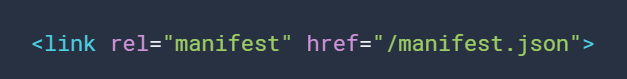
\includegraphics[scale=0.7]{img/include_manifest.png}
 %%       \caption{Einfache Einbindung des Manifests}
  %      \label{sourcecode:manifest_include}
        %https://developers.google.com/web/fundamentals/web-app-manifest?hl=en
%\end{figure}


\subsection{Service Worker für Offline-Funktionalität und Benachrichtigungen}
\label{chap:service_worker}

Damit die \ac{pwa} trotz fehlender Netzwerkverbindung funktioniert wird ein besonderer Mechanismus benötigt: der Service Worker. Mit ihm können Abhängigkeiten der App lokal gecached werden, so dass die Anwendung auch bei schlechter oder gar fehlender Netzwerkverbindung funktioniert. \cite[S. 7]{BeginningPWA}

Ein Service Worker ist ein von der UI seperiertat laufendes Hintergrundskript der Webanwendung, siehe Abbildung \ref{fig:serviceWorker}. Er wird genutzt um Bilder, Skripte, Styles oder ganze Seiten zu cachen. Bei bestehender Netzwerkverbindung führt er nötige Synchronisierungen durch. Nicht zuletzt ist er auch für das senden von Push-Notifications zuständig. \cite[S. 24]{BeginningPWA}

\begin{figure}[h]
        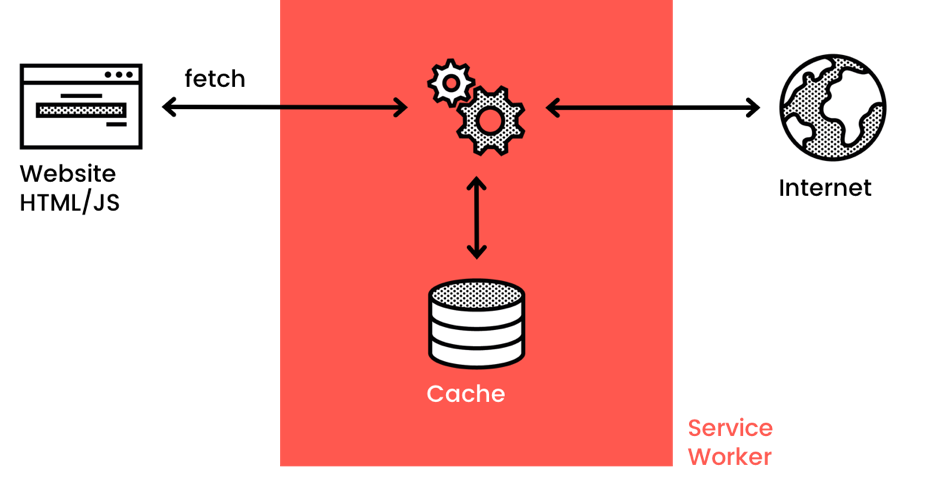
\includegraphics[width=\linewidth]{img/ServiceWorker-8a0968f1b295f1ff.png}
        \centering
        \caption{Konzept des Service Workers \cite{ServiceWorkerDiagramm}}
        \label{fig:serviceWorker}
\end{figure}


Alle verbreiteten Desktopbrowser wie Chrome, Firefox, Opera, Edge und mitterweile auch Safari unsterstützen das Service Worker Konzept. Der Mobile Chromebrowser unter Android unterstützt Service Worker bereits voll, während Safari unter iOS noch an diesem Feature arbeitet. \cite[S. 9]{BeginningPWA}


\subsection{Plattformen von eine \ac{pwa} aktuell unterstützen}
Das Projekt \textit{CanIUse} aggregiert Daten zu Webstandards des w3 Konsortiums und Browserdokumentationen. Es wird als Quelle für die Unterstützung von Features durch aktuelle Browser herangezogen.

Apples mobiler Browser Safari unterstützt eines der wichtigsten Features der \ac{pwa} noch nicht vollständig: das Web App Manifest. Allerdings wird der Service Worker vollständig unterstützt \cite{CanIUseWebManifest}. Wann und ob Safari die Unterstützung für das Manifest implementiert ist unklar und bleibt abzuwarten. Die aktuelle Teilunterstützung zeigt jedoch, dass sich Apple nicht grundsätzlich gegen die \ac{pwa} weigert.

 %Die Versionen zeigen aber eine stetig voranschreitende Integration der, erweitert den Funktionsumfang in den neusten Versionen von iOS. 

% https://medium.com/@firt/progressive-web-apps-on-ios-are-here-d00430dee3a7



% Source: https://developers.google.com/web/progressive-web-apps/desktop
Die Nutzung von \ac{pwa}s ist nicht ausschließlich auf Smartphones begrenzt. Wie normale Desktopprogramme werden Desktop \ac{pwa}s in einem eigenen Fenster gestartet. 
Der Unterschied zwischen den Bedienelementen nativer Desktopanwendungen und Desktop \ac{pwa}s ist ausschließlich farblicher Natur. Stark vereinfacht beschrieben, sind Desktop \ac{pwa}s Browserfenster ohne Tabs und Adressleiste. Durch die Nutzung von Service Workern, welche die Webanwendung cachen, sind auch Desktop \ac{pwa}s nicht an eine Netzwerkverbindung gebunden.

Grundsätzlich können Desktop \ac{pwa}s auf jedem Betriebssystem installiert werden, auf dem Google Chrome (Version größer 73) installiert werden kann: Windows, Mac, Linux und Chrome OS.
\cite{GooglePWADesktop}



\subsection{Grundlage der Webanwendung: JavaScript Laufzeitumgebung Node.js}

%NodeJSWebsiteAbout
Node.js ist eine open-source JavaScript Laufzeitumgebung für die Entwicklung skalierbarer Webanwendungen 
\cite{NodeJSWebsiteAbout}.
Selbst baut Node.js auf der V8-Engine auf, einer Laufzeitumgebung, die auch von Google Chrome genutzt wird 
%NodeJSRecepies
\cite[S. 1]{NodeJSRecepies}.
% PracitalNodeJS
Wegen zeitsparenden Features, wie automatischem Typecasting oder der Tatsache, dass Node.js alle Daten als Objekt behandelt, erfreut sich Node.js großer Beliebtheit 
\cite[S. 12]{PracitalNodeJS}.
Die Kombination mit dem Package Manager npm ermöglicht die einfache Installation und Nutzung von Modulen, um die Funktionalität der Plattform zu erweitern. 
\cite[S. 9]{NodeJSRecepies}.


\subsection{Frontend-Framwork Angular für die Entwicklung von Webanwendungen}

Angular ist ein open-source TypeScript basiertes Framework zur Entwicklung von Webanwendungen, welches Node.js nutzt.


%https://octoverse.github.com/projects
Mit über Achttausend Mitwirkenden Entwicklern (Angular CLI) beziehungsweise über Siebentausend Mitwirkender (Angular Framework) belegt das Angular Command Line Interface und das Angular Framework die Plätze 4 und 6 der größten Projekte auf Github. 
% https://octoverse.github.com/projects
\cite{OctoverseGitHubStatistics}

Das Framework arbeitet auf Basis von Komponenten. Ein Eingabefeld, Seite oder eine Liste werden in Angular als solche Komponenten seperat betrachtet. Auch in der Dateistruktur werden Komponenten stark getrennt. Jede Komponente besitzt beispielsweise ein eigenes CSS (oder SCSS) und HTML-File. Eine Komponente für eine Seite kann so auch eine oder sogar mehrere Listenkomponenten einbinden. Durch die Wiederverwendung von Code-Fragmenten in Komponenten wird der Programmcode sehr übersichtlich und strukturiert.

\begin{figure}[h]
        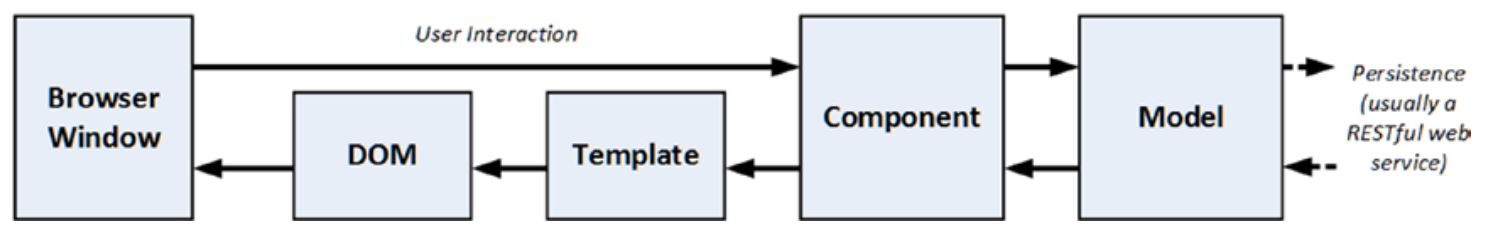
\includegraphics[width=\linewidth]{img/Angular_MVC.JPG}
        \centering
        \caption{MVC Konzept von Angular \cite[S. 35, Abbildung 3-4]{ProAngular}}
        \label{fig:angularmvc}
\end{figure}

Eine Angular Anwendung ist in drei Einheiten gegliedert:\\

\textbf{Model}\\ 
Enthält Logik für die Verwaltung von Daten, beispielsweise das Erstellen, Speichern oder Modifizieren. Dies kann über die Kommunikation mit einem Webserve via REST-API erfolgen. Das Model enhält keine Logik, um mit dem Nutzer zu interagieren.\\

\textbf{Component}\\
Enthält Logik für das Aktualisieren der Daten im Model aufgrund Nutzerinteraktion. \\

\textbf{Template}\\ 
Enthält Logik und Markup, um dem Nutzer Daten anzeigen zu können.

\cite{ProAngular}

\section{native Apps}


\subsection{Apple iOS} \label{chap:apple_ios}

iOS ist ein Betriebssystem, welches vom US-amerikanischen Technologiekonzern \textit{Apple, Inc.} im Rahmen des erstmalig vorgestellten \textit{iPhones} im Jahre 2007, damals noch unter dem Namen \textit{iPhone OS}, in Umlauf gebracht wurde. Stand heute läuft dieses Betriebssystem ausschließlich auf den Mobilgeräten des genannten Herstellers. Neben dem iPhone nutzt auch das Multimedia-Gerät \textit{iPod touch} das Betriebssystem iOS. Der Tabletcomputer \textit{iPad} wurde bis September 2019 ebenfalls über iOS betrieben, besitzt jedoch seit der Umstellung ein eigenes, an iOS stark angelehntes Betriebssystem \textit{iPadOS}.

\subsubsection{Entwicklung von iOS-Applikationen}

In seiner ersten Version stellte iPhone OS noch keinerlei Möglichkeit bereit, Anwendungen von Drittanbietern bereitzustellen sowie zu nutzen. Dies änderte sich bei der Umbenennung des Betriebssystems in iOS im Jahre 2008, welche auch ein Software-Update zur Folge hatte, in welchem diese Eigenschaft nun geboten wurde.

\paragraph{Programmiersprache: Apple \textit{Swift}}\mbox{}\\
In der Anfangszeit der Anwendungsentwicklung für iOS wurde die bereits für andere Zwecke entwickelte und vorhandene Programmiersprache \textit{Objective-C} als Standard gewählt. Dies änderte sich im Jahre 2014, als Apple bei seiner jährlichen Entwicklerkonferenz die hauseigene Programmiersprache \textit{Swift} vorstellte, welche Objective-C in der ganzheitlichen Anwendungsenwicklung rund um Apple-Geräte ablösen sollte. In der Anfangszeit von Swift war diese immer noch stark an den Vorgänger Objective-C angelehnt. Über die Zeit sank der Einfluss, jedoch ist Swift weiterhin abwärtskompatibel zu Objective-C, welche wiederum abwärtskompatibel zu C ist.

Bei Swift handelt es sich um eine objekt- und protokoll-orientierte Programmiersprache, welche in Ihren verschiedenen Anwendungsbereichen ihre Zugehörigkeit zu verschiedenen Programmierparadigmen aufweist. Diese stützt sich vor allem auf ihrer Behauptung, möglichst leicht verständlich für einen Menschen zu sein und vermeidet bekannte Probleme anderer, populärer objektorientierter Programmiersprachen, bspw. Dereferenzierung von \texttt{null}\textit{-Pointer-Exceptions}.

Neben der Entwicklung für alle Apple-Plattformen wird Swift unter anderem auch zur Back-End-Entwicklung genutzt. Laut einer Umfrage von \textit{StackOverflow} positioniert sich Swift auf Platz 14 der beliebtesten Programmiersprachen, basierend auf 8,1\% aller Stimmen.

\paragraph{Entwicklungsumgebung: Apple \textit{Xcode}}\mbox{}\\
\textit{Xcode} ist eine, ebenfalls von Apple entwickelte, sog. integrierte Entwicklungsumgebung (engl. \ac{ide}) und wird primär für die Entwicklung von Anwendungen mit der Programmiersprache Swift eingesetzt. Grundsätzlich ist Xcode, und somit auch die Programmierung mit Swift, Apple \textit{Mac}-Nutzern vorbehalten. Über die Zeit wurden weitere \acp{ide} entwickelt, welche Swift unterstützen, denen jedoch grundlegende, nachfolgend beschriebene Funktionalitäten von Xcode, fehlen. Zu nennen ist hier bspw. die Lösung \textit{AppCode} des Unternehmens \textit{JetBrains}.

Xcode unterstützt neben Swift auch die abwärtskompatiblen Programmiersprachen Objective-C, C, aber auch C++, Python, Ruby, sowie andere. Darüber hinaus bietet Xcode einen sog. \textit{Interface Builder}, mit welchem das Frontend über separate Ansichten (sog. \textit{Views}) vorbereitet werden kann. Dabei werden verschiedenste Komponenten bereitgestellt, welche via \textit{Drag'n'Drop} innerhalb der Ansichten platziert und optisch konfiguriert werden können. Auch Beziehungen zwischen den einzelnen Views können bereits hier angelegt werden. Ein Beispiel für die Nutzung des Interface Builders kann dem unten stehenden Screenshot entnommen werden.

\begin{figure}[h!]
	\centering
	\caption{Nutzung des Interface Builders in Xcode}
\end{figure}

% Erklärung des Screenshots
Die zusammengesetzten Komponenten können, ebenfalls über Drag-and-Drop in den Quellcode referenziert werden, um die Verhaltensweisen dieser programmatisch festzulegen. Ist die App in einem testreifen Zustand, kann diese direkt über Xcode emuliert werden. Es öffnet sich ein sog. \textit{Simulator}, welcher das Zielgerät mit der geöffneten Anwendung darstellt. Das Verhalten und etwaige, daraus resultierende Probleme, können somit erkannt werden, ohne, dass es ein tatsächliches, physikalisches Zielgerät bedarf. Eigenschaften, welche auf die Hardware-Komponenten des Geräts zugreifen (bspw. die eingebauten Kameras, den Bluetooth-Sensor, etc.) können mit Ausnahme der Netzwerkkarte nicht simuliert werden.

\paragraph{Softwaredesign-Muster \textit{Model-View-Controller}}\mbox{}\\ 
Apple empfiehlt als grundlegendes Prinzip für die App-Entwicklung mit Swift das Muster \textit{\ac{mvc}}, welches im Folgenden aufgeschlüsselt wird.

\begin{description}
	\item[Model] (dt. \textit{Modell} bezieht sich auf das Datenmodell und die datenbedingte Kommunikation innerhalb der Anwendung. Innerhalb von der iOS-Anwendungsentwicklung finden sich hier Quellcode-Abschnitte für die Kommunikation der App mit einer potenziellen \acs{api}, Code für die Definition und Bereitstellung von persistentem Speicher sowie die Handhabung der dadurch entstehenden Daten. Auch im Quellcode verwendete Konstanten sind dem Modell zuzuschreiben.
	\item[View] (dt. \textit{Präsentation}) bezieht sich auf die Frontend-Komponenten der Anwendung. Alle durch den Interface Builder spezifizierten Eigenschaften sind der Präsentation zuzuschreiben, also jegliche Komponenten, frontend-basierte Klassen sowie Animationen.
	\item[Controller] (dt. \textit{Steuerung}) beinhaltet die spezifische Verhaltenslogik der Anwendung bei Interaktion mit dieser durch den Nutzer. Vereinfacht formuliert bestimmt dieser, welche Funktionalität zu welcher Zeit auf Basis welches Verhaltens ausgeführt wird. Diese ist ebenfalls für die Kommunikation zwischen dem Modell und der Präsentation zuständig.
\end{description}

Die Kooperation der einzelnen Komponenten dieses Musters lässt sich anhand der unten stehenden Abbildung erläutern.

\begin{figure}[h!]
	\centering
	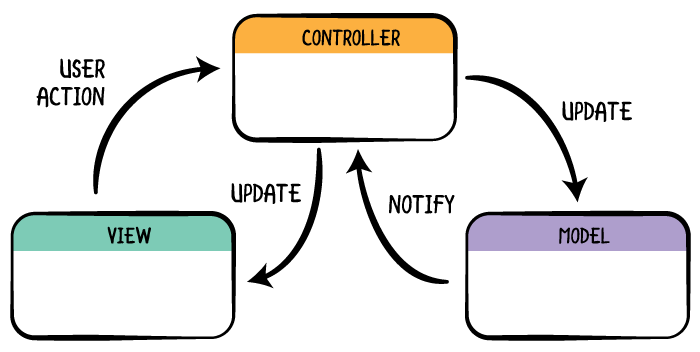
\includegraphics[width=0.5\linewidth]{img/mvc}
	\caption{Zusammenspiel des \ac{mvc}-Musters}
\end{figure}

% Erklärung MVC-Grafik

Technisch wird dieses Muster durch die Verknüpfung der einzelnen (durch den Interface Builder bereitgestellten oder erstellten) Views mit spezifischen, sog. \textit{View Controllern} realisiert. Durch eine Aktion des Nutzers auf dem View wird die entsprechende Funktionalität über den View Controller bereitgestellt. Dieser kann dann ebenfalls Funktionen ausführen, welche durch das Modell bereitgestellt werden, falls die Aktion dies bedarf. Die entsprechenden Klassen der View Controller sind Unterklassen der einzelnen, spezifischen Views, welche deren vorgesetzte Basisfunktionalitäten um die gewünschten Funktionen des Entwicklers erweitern.

\paragraph{Vorbereitung der Projektumgebung}\mbox{}\\
Bei der Erstellung eines neuen Projektes innerhalb von Xcode wählt der Entwickler bereits zu Beginn bestimmte Spezifikationen für die zu entwickelnde Anwendung. Da Swift auch für andere Betriebssysteme von Apple zur Anwendungsentwicklung genutzt wird, gehört die Spezifizierung des Anwendungsbereiches (hier: iOS) sowie des grundlegenden Aufbaus der App zu den Vorbereitungsmaßnahmen der Projektumgebung. Dieses Dialogfenster kann aus dem unten stehenden Screenshot entnommen werden.

\begin{figure}
	\centering
	\caption{Dialogfenster zum Anlegen eines neuen Projektes (Xcode)}
\end{figure}

Letztere bereiten verschiedene Dateitypen innerhalb der Umgebung vor, bspw. verschiedene Ansichten mit bereits integrierter Navigation, welche bei einer Anwendung mit nur einer Ansicht nicht zu tragen kommen. Im zweiten Schritt der Projektvorbereitung trifft der Entwickler Entscheidungen über Projektverzeichnis, -namen und -sprache sowie über weitere Projektkomponenten, welche für die Anwendung von Bedarf wären.

Alle hier getroffen Schritte können auch manuell bzw. im Nachgang der Projekterstellung angelegt werden. Grundsätzlich sind die Dateien und Quellcodezeilen, welche durch die genannten Vorbereitungsmaßnahmen automatisch generiert werden, unabdingbar für die Realisierung des Projekt und können somit für eine effizientere Arbeit des Entwicklers sorgen.

\paragraph{Struktur des initialen Entwicklungsverzeichnisses}
Bereits zu Anfang befinden sich bestimmte Dateien im Entwicklungsverzeichnis, welche sich grundsätzlich in jeder iOS-Anwendung benötigt werden. Diese werden im Folgenden beschrieben.

\begin{description}
	\item[\texttt{AppDelegate.swift}] ist der Eintrittspunkt der App. Dieser ist zuständig für das Verhalten der App, wenn diese (zum ersten Mal) geöffnet, geschlossen oder in den Hintergrund gerückt (d.\ h. inaktiv gesetzt) wird. Diese Datei ist vor allem dann von Interesse, wenn die Anwendung auch außerhalb ihrer Aktivität bestimmte Funktionen ausführt, bspw. also bei Musik-Anwendungen oder Stoppuhren. Aufgrund der automatischen Bereitstellung von Core Data zu Anfang des Projektes ist hier auch das Grundgerüst des \textit{Persistent Service} zu finden.
	\item[\texttt{SceneDelegate.swift}] ähnelt dem \texttt{AppDelegate} sehr, bezieht sich jedoch auf das Verhalten der Ansicht(-en) der Anwendung. Diese wird benötigt, da seit iOS-Version 13 auch mehrere offene Instanzen derselben App möglich sind, welche jedoch immer den aktuellsten Zustand darstellen sollen, unabhängig von der gerade aktiv laufenden Instanz. In Form einer Analogie aus der Web-Entwicklung kann man den \texttt{SceneDelegate} als die oberste Hierarchie der \textit{Frontend}-Steuerung bezeichnen, während das \textit{Back End} über den \texttt{AppDelegate} orchestriert wird.
	\item[\texttt{ViewController.swift}] ist einer von beliebig vielen möglichen Controllern, welche direkte Anbindung zu einer oder mehreren Ansichten hat. Dieser beinhaltet Konfigurationen der verschiedenen Komponenten der Ansicht und spezifiziert auch das Verhalten der Ansicht, wenn auf diese oder von dieser gewechselt wird.
	\item[\texttt{Main.storyboard}] ist das Gegenstück zu den \texttt{ViewController}. In Form eines sog. \textit{Interface Builders} können verschiedene Ansichten und deren Verknüpfungen via \textit{Drag-and-Drop} erstellt werden. Jede Ansicht wird mit genau einem \texttt{ViewController} versehen, welcher die Steuerung der definierten Elemente übernimmt. Grundsätzlich ist es auch möglich, vollständig ohne Interface Builder auszukommen. Die initiale Konfiguration der Positionen und der weiteren optischen Eigenschaften wird dann ebenfalls über den entsprechenden \texttt{ViewController} gehandhabt, wobei dies einen deutlich höheren Programmieraufwand aufweisen könnte. Neben des \texttt{Main.storyboard} existiert auch ein \texttt{LaunchScreen.storyboard}, welcher beim Laden der Anwendung ausgeführt wird.
	\item[\texttt{Assets.xcassets}] beinhaltet das App-Logo, welches im Menü des Mobilgerätes angezeigt wird. Dieses muss in fest definierten Größen bereitgestellt werden, wird jedoch an dieser Stelle vernachlässigt. Darüber hinaus können hier auch alle weiteren Grafiken, etc., abgelegt werden, welche innerhalb der App genutzt werden, um für eine ordnungsgemäße Skalierung der Symbole je nach Bildschirmgröße des Endgeräts zu gewährleisten.
	\item[\texttt{Info.plist}] ist eine allgemeine Konfigurationsdatei. Diese wird u.a. für Berechtigungen genutzt, welche die Anwendung außerhalb ihres eigenen Handlungsspielraums haben soll, bspw. die Nutzung der eingebauten Kameras, des GPS-Standortes des Geräts, die Berechtigung, Benachrichtigungen anzuzeigen, etc.
	\item[\texttt{to\_do.xcdatamodeld}] stellt die Konfigurationsdatei des Persistent Service dar, sofern dieser im Dialogfenster aktiviert wurde. In dieser werden Entitäten angelegt, mit möglichen Relationen versehen und für die Verwendung innerhalb der App exportiert.
\end{description}

\subsubsection{Vertrieb von iOS-Applikationen}
Der mit iOS 2.0 (Nachfolger von iPhone OS) ins Leben gerufene Apple \textit{App Store} ist die einzige offizielle Bezugsstelle für iOS-Applikationen. Somit ist es auch der am meisten verwendete Marktplatz, in welchem Entwickler und Unternehmen ihre Anwendung kostenlos sowie kostenpflichtig zum Download anbieten.

Zunächst ist die Anmeldung des Entwicklers als \textit{Apple Developer} im Vorhinein erforderlich. Ohne diese könnte die Anwendung zwar programmiert und innerhalb der Entwicklungsumgebung getestet, jedoch nicht auf tatsächlichen iOS-Geräten getestet und zum Download freigegeben werden. Dies hat sowohl sicherheitstechnische als auch wirtschaftliche Gründe, welche hier nicht weiter diskutiert, jedoch für die Evaluation der Entwicklungsfreiheit in Betracht gezogen werden. Letzteres erkennt man vor allem an der Tatsache, dass die Verbreitung von Anwendungen über den \textit{App Store} kostenpflichtig ist.

% Evtl. Quelle für die App-Publikation (iOS) finden und zitieren
Der genaue Prozess der Publikation von iOS-Applikationen kann im Rahmen dieser Arbeit nicht nachvollzogen werden, da keine Möglichkeit der tatsächlichen Bereitstellung der zu entwickelnden Beispielanwendung vorliegt.

\subsubsection{Nutzung von iOS-Applikationen}
Wie im vorigen Abschnitt erwähnt werden iOS-Anwendungen über den App Store bezogen. Auf weitere, inoffizielle und teils nonkonforme Praktiken wie das sog. \textit{Jailbraking} des Gerätes, um auch nicht-authorisierte Anwendungen herunterladen und nutzen zu können, wird hier nicht eingegangen.

Der iOS-Nutzer sucht über den App Store die gewünschte App und lädt diese herunter. Für diesen Prozess ist eine sog. \textit{Apple ID}, also ein Benutzerkonto bei Apple vonnöten. Sollte die gewünschte App kostenpflichtig sein, so müssen Kreditkarten- oder anderweitige, valide Zahlungsdaten dem Konto hinterlegt sein. Der Nutzer bestätigt den Kauf bzw. erstmaligen Download über das Benutzerkontenpasswort oder eine gerätespezifische Authentifizierungsmethode (bspw. Fingerabdruck-Erkennung via \textit{Touch ID} oder Gesichtserkennung via \textit{Face ID}, sofern vorhanden). Daraufhin startet der Download. Die App kann über ihr korrespondierendes App-Symbol, welches nun auf dem Menü-Bildschirm des Geräts erscheint, geöffnet werden.

Falls die App in einer nun aktuelleren Version vorliegt, wird diese entweder über den App Store automatisch im Hintergrund neu heruntergeladen. Andernfalls kann der Nutzer diesen Schritt auch manuell über den App Store in Kraft setzen.



\subsection{Android}

\textbf{Entwicklung}

%Android apps are written in Java and use various Java application program interfaces (APIs).
%Because you’ll want to write your own apps, but may be unfamiliar with the Java language and these
%APIs, this book teaches you about Java as a first step into Android app development. It provides you
%with Java language fundamentals and Java APIs that are useful when developing apps.

Native Android Anwendungen werden in Java entwickelt. Durch die Nutzung der zahlreichen APIs wird aus einem Java Programm eine native Android App.
\cite[S. 1]{JavaForAndroid}
Mittlerweile wird die teilweise veraltete Java-Syntax graduell durch die modernere Programmiersprache Kotlin abgelöst.
\cite{KotlinAndroid}


%Kotlin is a free and open source project under the Apache 2.0 license
%https://developer.android.com/kotlin

%https://kotlinlang.org/docs/reference/android-overview.html

Meist werden Android Apps mithilfe der Entwicklungsumgebung Android Studio entwickelt, welches auf der IntelliJ IDE von JetBrains aufbaut, aber von Google weiterentwickelt wird. Die IDE bietet Entwicklern unter anderem einen visuellen Layout-Editor und eine Vielzahl von Android Emulatoren zum Testen der Apps auf verschiedenen Android Versionen und unterschiedlicher Hardware. Dafür wird jedoch performante Hardware zum Entwickeln benötigt: 8 Gigabyte Arbeitsspeicher oder mehr ist die Empfehlung der Herausgeber. \cite{AndroidStudio}

\textbf{Vertrieb}

Die meisten Apps beziehen Nutzer über den Google Play Store, einem Onlineshop für kostenlose und kostenpflichtige Android Anwendungen. 
Updates werden ebenfalls über den Play Store installiert. Alternativ kann ein Nutzer eine App in Form einer \texttt{.apk}-Datei installieren. Dieser Weg bleibt jedoch aufgrund der Umständlichkeit und bedenklicher Sicherheit der App weitestgehend ungenutzt.




\subsection{Android}

\textbf{Entwicklung}

%Android apps are written in Java and use various Java application program interfaces (APIs).
%Because you’ll want to write your own apps, but may be unfamiliar with the Java language and these
%APIs, this book teaches you about Java as a first step into Android app development. It provides you
%with Java language fundamentals and Java APIs that are useful when developing apps.

Native Android Anwendungen werden in der Regel in Java entwickelt. Durch die Nutzung der zahlreichen APIs wird aus einem Java Programm eine native Android App.
\cite[S. 1]{JavaForAndroid}
Mittlerweile wird die teilweise veraltete Java-Syntax graduell durch die modernere Programmiersprache Kotlin abgelöst.
\cite{KotlinAndroid}


%Kotlin is a free and open source project under the Apache 2.0 license
%https://developer.android.com/kotlin

%https://kotlinlang.org/docs/reference/android-overview.html

Meist werden Android Apps mithilfe der Entwicklungsumgebung Android Studio entwickelt, welches auf der IntelliJ IDE von JetBrains aufbaut, aber von Google weiterentwickelt wird. Die IDE bietet Entwicklern unter anderem einen visuellen Layout Editor und eine Vielzahl von Android Emulatoren zum Testen der Apps auf verschiedenen Android Versionen und unterschiedlicher Hardware. Dafür wird jedoch performante Hardware zum Entwickeln benötigt: 8 Gigabyte Arbeitsspeicher oder mehr ist die Empfehlung der Herausgeber. \cite{AndroidStudio}

\textbf{Vertrieb}

Die meisten Apps beziehen Nutzer über den Google Play Store, einem Onlineshop für kostenlose und kostenpflichtige Android Anwendungen. 
Updates werden ebenfalls über den Play Store installiert. Alternativ kann ein Nutzer eine App in Form einer \texttt{.apk}-Datei installieren. Dieser Weg bleibt jedoch aufgrund der Umständlichkeit und unbekannten Sicherheitsprüfung der App weitestgehend ungenutzt.

		
	\chapter{Wissenschaftliches Framework}
		\label{chap:wissenschaftliches_framework}
		%===========================================================================
%	III. Wissenschaftliches Framework
%===========================================================================

Die Grundlage für eine adäquate Bewertung der zu entwickelnden mobilen Anwendungen bildet die Definition beidseitig anwendbarer, quantifizierender Kriterien. Die Notwendigkeit hierin begründet sich darin, dass kein allgemein anerkannter Kriterienkatalog für die Pauschalisierung von Softwarequalität existiert. Viel eher benötigen unterschiedliche Projekte mit unterschiedlichen Schwerpunkten eine unterschiedlich definierte Definition der entsprechenden Gesichtspunkte.

Wie zuvor erwähnt wird die Forschungsfrage, ob \acp{pwa} native Apps langfristig ersetzen können, vor allem auf Basis der Umsetzbarkeit in der Entwicklung evaluiert. Umgekehrt könnten ähnliche Fragestellungen anhand wirtschaftlicher Aspekte begründet werden (bspw. Anzahl der benötigten Entwickler, preislicher Rahmen, Profitmöglichkeiten, etc.). Bei der Einfachheit der Beispielanwendung haben solche Aspekte jedoch kaum Bedeutung. Ebenfalls in Betracht gezogen werden muss die Tatsache, dass die Verfasser dieser Studienarbeit keine erfahrenen Entwickler ersetzen, weswegen auch quantifizierende Kriterien wie die Dauer der Entwicklungszeit, etc., keine Anwendung in der zugrunde liegenden Bewertung finden können. Gleiches gilt ebenfalls für die nur empirisch evaluierbaren Punkte der Nutzung seitens der Anwender (z.B. Intuitivität, Benutzerfreundlichkeit, Anspruch der Gestaltung, etc.), da eine solche Studie den Rahmen dieser Arbeit verlassen würde.

Bezüglich der Umsetzung in der Entwicklung lassen sich jedoch mehrere Kriterien aufstellen, die zur Beantwortung (oder zumindest Lenkung) der Forschungsfrage beitragen können. Die Definition der allgemeinen technischen Architektur in Kapitel \ref{chap:architektur} der zu entwickelnden Mobilanwendung geschieht unter Berücksichtigung der Kriterien, um eine neutrale Vergleichbarkeit zu ermöglichen.

\section{Vorgehen bei der Bewertung}
Um die Entwicklungen der Angular-\ac{pwa} und der nativen iOS-App zu vergleichen, wird die im Folgenden beschriebene Kriteriengewichtung (siehe Tabelle \ref{tab:punktekatalog}) verwendet. Einzelne Kriterien werden anhand Tabelle \ref{tab:verrechnungspunkte} bewertet und die Verrechnungspunkte anschließend über alle betrachteten Kriterien aufsummiert.

\begin{table}[h!]
	\centering
	\begin{tabular}{|c|c|c|c|c|c|}
		\hline 	
			\textbf{Bewertung} & $--$ & $-$ & \Circle & $+$ & $++$ \\ 
		\hline 
			\textbf{Beschreibung} & schlecht & eher schlecht & neutral & eher gut & gut \\ 
		\hline 
			\textbf{Verrechnungspunkte} & $-2$ & $-1$ & $0$ & $1$ & $2$ \\ 
		\hline 		
	\end{tabular} 
	\caption{Verrechnungspunkte} \label{tab:verrechnungspunkte}
\end{table}

Das Ergebnis ist eine Evaluationsmatrix, welche als Netzdiagramm dargestellt die bewerteten Kriterien einzeln visualisiert und eine Gesamtbewertung pro Technologie liefert. In diese fließen die Kriterien einzeln ein und bilden ein Gesamtbild. Die Gewichtung der Kriterien ist in Tabelle \ref{tab:punktekatalog} dargestellt.

\begin{table}[h!]
	\centering
	\begin{tabular}{|l|c|}
		\hline
		Kriterium              & Gesamtanteil \\
		\hline
		\multicolumn{2}{c}{Anwendung}     \\
		\hline
		Plattformabhängigkeit   & 10\%         \\
		Installation           & 5\%          \\
		Speicherzugriff        & 5\%          \\
		Speicherbedarf         & 5\%          \\
		Aktualisierbarkeit     & 5\%          \\
		Konsistenz des Designs & 5\%         \\
		
		\hline
		\multicolumn{2}{c}{Entwicklung}     \\
		\hline
		Bibliotheken           & 10\%         \\
		Umsetzung              & 20\%         \\
		Testbarkeit            & 10\%         \\
		Vorausgesetzte Entwicklungserfahrung    & 10\%         \\
		\hline
		\hline
		Summe                  & 100\%        \\
		\hline
	\end{tabular}
	\caption{Kriteriengewichtung} \label{tab:punktekatalog}
\end{table}

\section{Betrachtete Aspekte der Entwicklung}
Bei der Evaluation soll auf verschiedene Aspekte beider Projekte eingegangen werden. Diese lauten wie folgt:
\begin{description}
	\item [Anwendung]
		Die Kriterien zur Anwendung (bzw. App) beziehen sich auf die Eigenheiten der Apps, darunter die Installation, die Aktualisierung und die Plattformabhängigkeit.
		
	\item [Entwicklung]
		Kriterien der Entwicklung beziehen sich auf die Programmierung und Umsetzung der funktionalen und nicht-funktionalen Anforderungen.
			
\end{description}


Grundsätzlich gibt es einen Punktabzug, wenn der Nutzer grundlegenden Funktionen explizit zustimmen muss. Das Idealbild ist eine sofort nutzbare Anwendung, die ohne weitere Zwischenschritte den kompletten Funktionsumfang besitzt.

\section{Betrachtete Kriterien}
Die einzelnen Kriterien aus der Evaluationsmatrix werden nun genauer definiert:

\begin{description}
	\item [Plattformabhängigkeit] 
		  Unterstützt die Anwendung mehrere Plattformen, also beispielsweise Android und iOS wird dies als gut bewertet. Ist die Anwendung auch auf Desktop-Computern oder Tablets nutzbar, gibt dies ebenfalls eine positive Bewertung.
		  
	\item [Installation]
	      Die App sollte ohne mehrere Zwischenschritte nutzbar sein. Ist die Installation zu kompliziert, führt dies zu Punktabzug.

	      Es fließt mit ein, wie viel Aufwand betrieben werden muss, um die App einem Publikum zur Verfügung zu stellen. Dieser Aufwand ist idealerweise gering und im Interesse des Entwicklers.

	\item [Speicherzugriff]
	      Anwendungen müssen Daten speichern können, um dem Nutzer einen Mehrwert zu bieten. Die Größe der zu speichernden Daten ist bei diesem Vergleich auf einige Kilobyte begrenzt. Gibt es die Möglichkeit Dateien abzulegen, ist dies positiv zu werten. Idealerweise können Daten in gängigen Formaten (beispielsweise \acsu{json}, \acsu{csv}, \acsu{xml} oder Plaintext) gespeichert werden.
	      Können Daten nur temporär und nicht persistent gespeichert werden, führt dies zu starkem Punktabzug. Muss der Nutzer dem Speichern von Daten aktiv zustimmen, stört dies die Nutzungserfahrung und ist daher negativ zu werten.

	\item [Speicherbedarf]
	      Der Speicherplatz eines Smartphones ist deutlich kleiner, als der eines Desktop-Computers. Bestenfalls ist die Anwendung nur einige Megabyte groß und kann so schnell über eine mobile Datenverbindung installiert und upgedatet werden \cite{AppleMaxAppSize} \cite{GoogleMaxAppSize}. 
	      Hoher Speicherverbrauch führt zu Punktabzug, wohingegen geringer Speicherverbrauch positiv bewertet wird. Der Verbrauch ist unter den einzelnen Plattformen relativ zu bewerten.

	\item [Aktualisierbarkeit]
	      Idealerweise kann die Installation von Updates vom Entwickler kontrolliert werden. Schnelle Updatezyklen sind wünschenswert, da in der Praxis dadurch schnell Sicherheitslücken und Bugs behoben werden können. Wenn ein Nutzer sich aktiv gegen Updates weigern kann, oder diese manuell installieren muss, könnte dies für Kompatibilitätsprobleme mit Webschnittstellen oder Sicherheitsprobleme sorgen und führt deshalb zu Punktabzug.

	      Der Aufwand der betrieben werden muss, um Updates einzubringen, wird mitevaluiert. Je schneller Updates flächendeckend auf den Geräten der Nutzer landen, desto höher die Punktzahl.

	\item [Design]
	      Idealerweise sieht die Anwendung auf verschiedenen Geräten identisch aus. Grundsätzlich wird erwartet, dass Schriften, Farben und Größenverhältnisse auf unterschiedlichen Geräten und gegebenenfalls unterschiedlichen Browsern ein konsistentes Bild ergeben.
	      Eine skalierende Nutzeroberfläche ist wünschenswert. Anzeigefehler, wie bspw. überlappende Objekte, fehlerhafte Elemente oder fehlende Schriftarten, führen zu Punktabzug. Auch der Aufwand, welcher betrieben werden muss, um das Nutzerinterface skalierbar zu gestalten, fließt in die Bewertung mit ein.

%	\item[Nutzerfreundlichkeit]
	%      Dem Nutzer sollte zu jedem Zeitpunkt klar sein, wie die Anwendung installiert, gestartet und deinstalliert werden kann. Ist dies nicht gewährleistet werden Punkte abgezogen.
	      
	 %     Dieses Kriterium bezieht sich auf die Technologie native App oder \ac{pwa}, nicht jedoch auf Nutzerfreundlichkeit im Sinne der Ergonomie, welche das User Interface aufweist. Diese obliegt vollständig dem Entwickler und ist für diesen Vergleich daher nicht aussagekräftig.

	\item[Bibliotheken]
		Um den Programmier- und Wartungsaufwand zu minimieren, greifen Entwickler auf Bibliotheken zurück, welche Lösungen für verbreitete Probleme anbieten.
		 In der Evaluation werden Bibliotheken von Open-Source-Organisationen und ggf. Bibliotheken des Plattformanbieters (bpsw. Apple, Google, Mozilla, etc.) betrachtet. In die Bewertung fließt ein, wie komplex sich der Prozess für Entwickler darstellt, um Bibliotheken zu nutzen und zu installieren. 

	\item[Umsetzbarkeit]
		Das bewertete Kriterium der Umsetzbarkeit beinhaltet die Komplexität und die Herausforderungen bei der Implementierung der funktionalen und nicht-funktionalen Anforderungen. Sind Anforderungen aufgrund plattformspezifischer Einschränkungen nicht oder nur beschränkt umsetzbar, führt dies zu Punktabzug. Es wird angenommen, dass die Anforderungen mit allen etablierten Technologien für die App-Entwicklung vollständig umgesetzt werden können.
		
		Bietet die Plattform im Umkehrschluss einfache und schnelle Mechanismen zur Umsetzung der Anforderungen, fließt dies positiv in die Wertung mit ein.
		
	\item[Testbarkeit]
		Das Testen von Software gehört zu den Grundlagen der Qualitätssicherung. Es wird erwartet, dass es einfache und schnelle Methoden zum Testen der Apps nach einer Änderung im Quellcode gibt.
	
	\item[Vorausgesetzte Entwicklungserfahrung]
		Es soll eingeschätzt werden, wie hoch die Einstiegshürde für die Entwicklung der jeweiligen Technologie ist. Die Anzahl und Komplexität der Tools fließt in die Bewertung mit ein. Es wird angenommen, dass die Entwicklung mit einem einzigen Werkzeug für den Entwickler einfacher ist, als das Bedienen mehrerer komplexerer Entwicklungstools. Gibt es grafische Oberflächen für viele Entwicklungsschritte ist dies positiver zu bewerten, als das Arbeiten mit Skripten und der Kommandozeile.
		
\end{description}


		
	\chapter{Architektur}
		\label{chap:architektur}
		%===========================================================================
%	IV. Architektur
%===========================================================================

Die hier zu entwickelnde Anwendung dient zum Anlegen und Verwalten von Aufgaben der Nutzer. Somit löst sie die sogenannte, analoge \textit{To-Do-Liste} ab. Dabei hat die Anwendung (und somit auch die Studienarbeit) keinen Anspruch auf Innovationsdarbietung. Die Begründung der dieses speziellen Entwicklungsbeispiels liegt darin, dass eine To-Do-Listen-Anwendung ein großes Spektrum von Funktionen abbilden kann. Dieses Spektrum reicht von grundlegenden Funktionen (bspw. dem bloßen Anlegen von Aufgaben) bis zu komplexeren Inhalten (bspw. automatischen Push-Notifications über unerledigte oder überfällige Aufgaben). Diese design- und architekturbedingenden Entscheidungen werden im Folgenden definiert und näher beschrieben.

Die Beschreibung der Architektur einer zu entwickelnden Applikation ist eine maßgebende Disziplin im Software-Engineering-Prozess. Dieser Prozess geschieht vor Beginn der Implementierung und ermöglicht, bezogen auf den Umfang dieser Studienarbeit, die Vergleichbarkeit der Applikation hinsichtlich der relevanten Entwicklungsplattformen. Der Umfang sämtlicher Software-Engineering-Prozesse wird grundsätzlich in großen Entwicklerteams praktiziert. Diese gehen der Entwicklung meist komplexer und skalierbarer Anwendungen nach. Im Vergleich dazu ist die hier zu entwickelnde Mobilanwendung lediglich Mittel zum Zweck für die Beantwortung der Forschungsfrage. Das Entwicklungsteam der To-Do-Anwendung besteht aus zwei Personen, welche sich im Rahmen dieser Arbeit autark mit unterschiedlichen Entwicklungsplattformen beschäftigen.

Dies sorgt dafür, dass sich lediglich eine abgespeckte Form des Software-Engineering auf dieses Projekt anwenden lässt. Konkret bedeutet dies, dass keine spezifischen Aussagen über den Software-Prozess bzw. über das Entwicklungsmodell (Wasserfall-Modell, iteratives Modell, etc.) gemacht werden. Dies würde sich hinsichtlich des verhältnismäßig geringen Entwicklungs- und Wartungsaufwands der App kontraproduktiv auf die Zielorientierung auswirken. Umso wichtiger ist die Definition funktionaler sowie nicht-funktionaler Anforderungen, welche daraufhin näher erläutert und spezifiziert werden. Auch die Interaktion zwischen Nutzer und Anwendung muss für eine vergleichende Entwicklung definiert werden. Die zeitlichen und komponentenabhängigen Abläufe innerhalb der App gehören ebenfalls zu den Bestandteilen der Architektur. Letztere beiden Punkte werden im Rahmen des sog. \textit{Systems Modelling} definiert. Darüber hinaus werden auch optische Aspekte und Verhaltensweisen des \ac{ui} abgegrenzt.


\section{Anforderungsdefinition} \label{sec:4-anfoderungen}
Die Funktionalität der Anwendung wird zunächst über die Anforderungsdefinition näher beschrieben. Diese kann auf allgemeine Funktionsweisen der App (nicht-funktionale Anforderungen), sowie auf spezifische, technische Charakteristika abgegrenzter Bereiche der Anwendung (funktionale Anforderungen). Grundsätzlich gilt es, nicht-funktionale Anforderungen im Laufe der Anforderungsdefinition in meist mehrere funktionale Anforderungen zu überführen \cite{Garidis}, da diese qualifizierbarer sowie quantifizierbarer Natur sind und somit ebenfalls für eine bessere Vergleichbarkeit der zu entstehenden Anwendungen beitragen könnten.

\subsection{Nicht-Funktionale Anforderungen} \label{subsec:non-functional}
Die folgenden nicht-funktionalen Anforderungen beziehen sich auf Teile der Anwendung, welche jedoch abstrakter Natur sind, weswegen sie zunächst zu nicht-funktionalen Anforderungen gezählt werden müssen. Aufgrund der Formulierung werden diese Anforderungen auch als \textit{Nutzeranforderungen} (engl. \textit{User Requirements}) bezeichnet und stehen den spezifischeren, technisch versierteren \textit{Systemanforderungen} (engl. \textit{System Requirements}) gegenüber \cite{Garidis}.
\begin{description}
    \item[Anlegen, Auflisten, Bearbeiten und Löschen von Aufgaben] Die Anwendung ermöglicht es, Aufgaben hinzuzufügen. Die hinzugefügten Aufgaben werden aufgelistet. Bei Bedarf soll der Inhalt der Aufgabe nachträglich abgeändert werden können. Ebenfalls ist es möglich, die Aufgabe aus der Ansicht innerhalb der Anwendung zu entfernen.
    \item[Aufgaben bestehen nach Neustart der Anwendung bei] Wird die Applikation (gewollt und ungewollt) neu gestartet, bildet sie nach Neustart dieselben Aufgaben und Einstellungen wie zuvor ab.
    \item[Priorisierung der Aufgaben möglich] Bei Bedarf ist es möglich, einer bestimmten Aufgabe einen gesonderten Stellenwert zuzuweisen.
    \item[Benachrichtigungen über nicht-erledigte und überfällige Aufgaben] Der Nutzer wird unabhängig vom Status der Applikation oder des Smartphones (d.h. online/offline, geöffnet, im Hintergrund oder geschlossen bzw. gesperrt oder entsperrt) über nicht-erledigte und überfällige Aufgaben benachrichtigt.
\end{description}
Neben dieser Art der nicht-funktionalen Anforderungen koexisitieren jene, welche zwar ebenfalls abstrakt und allgemein gehalten sind, jedoch keinen Bedarf resp. keine Möglichkeit zur weiteren Spezifizierung an dieser Stelle des Prozesses aufweisen.
\begin{description}
    \item[Bereitstellung der Anwendung für mehrere Plattformen] Die Anwendung ist nicht nur auf einer Plattform verfügbar, sondern kann auf Geräten unterschiedlicher Betriebssysteme installiert und verwendet werden.
    \item[Aussehen und Verhalten sind deckungsgleich] Unabhängig davon, welche Plattform genutzt wird, ist die Interaktion zwischen dem Nutzer und der Anwendung annähernd identisch. Davon ausgenommen sind Aspekte, welche auf der entsprechenden Plattform nicht oder nur mit unverhältnismäßigem Aufwand erreicht werden können.
    \item[zeiteffizienter Entwicklungsprozess] Um auch einen entwicklungstechnischen Vergleich ziehen zu können, soll die Anwendung in einer dem Projekt angemessenen Zeit vollständig entwickelt werden können.
\end{description}
Die Problematik nicht-funktionaler Anforderungen im Bezug auf realistisch zu betrachtende Entwicklungsprojekte kann hier interpretiert werden. Vor allem bei eher unerfahrenen Entwicklern (zu welchen sich das Entwicklerteam dieses Projektes zu zählen erlaubt) sind bestimmte Tendenzen unklar. Dazu gehören bspw. das Bewusstsein über die Realisierbarkeit bestimmter Komponenten sowie die zeitliche Aufwandseinschätzung. Diese Störfaktoren werden im Laufe der Arbeit versucht, entkräftet zu werden und sind in die Evaluation der Forschungsfrage kritisch einzubeziehen.

\subsection{Funktionale Anforderungen}
Nichtsdestotrotz ist die Spezifizierung der in Abs. \ref{subsec:non-functional} eingangs definierten nicht-funktionalen Anforderungen noch ausstehend. Zur Unterstützung der Lesbarkeit werden diese in Reihenfolge der nicht-funktionalen Anforderungen abgehandelt.

\begin{description}
    \item[Bereitstellung klassischer \acs{crud}-Operationen] Sog. \textit{\ac{crud}}-Operationen greifen auf das Datenmodell der Anwendung zu. Diese erlauben die Manipulation der Daten auf Basis der gewünschten Operation. Diese Operationen sind unabhängig voneinander zu definieren und sinnvoll in den Verwendungsprozess der App einzubauen. Man spricht hier auch von sog. \ac{crud}-\textit{Endpoints}, welche vereinfacht als statische Funktionen beschrieben werden können.
    \item[Listendarstellung] Die Aufgaben sollen grundsätzlich in einer sortierten Liste dargestellt werden. Die Liste besteht aus individuellen Elementen, welche jeweils eine Aufgabe darstellen. Jene \ac{crud}-Operationen, welche speziell auf eine bestimmte Aufgabe angewandt werden sollen, finden ihre Aktivierung ebenfalls über ihre entsprechenden Elemente.
    \item[Bereitstellung eines Persistent Services] Bei Ausführen der zuvor definierten \ac{crud}-Operationen werden die Daten nicht nur in den flüchtigen Arbeitsspeicher des Smartphones geschrieben, sondern zugleich auch auf einen der Applikation zugewiesenen Festspeicher. Diese idealisierte Datenbank gleicht dem Datenmodell für die \ac{crud}-Operationen und wird somit bei jeder Ausführung dieser aktualisiert bzw. beansprucht.
    \item[Definition einer Hierarchie für Aufgaben] Eine hierarchische Struktur der Daten soll ermöglichen, bestimmte Aufgaben seitens der Anwendung anders zu behandeln als andere. Durch das Setzen eines sog. \textit{Flags} können die Aufgaben entsprechend der Hierarchiestruktur bestimmte Zustände übergeben bekommen, konkret eine hervorgehobene optische Darstellung innerhalb der \ac{ui} sowie die Präsentation an Anfang der Liste (Eingriff in die Sortierung der Aufgaben)
\end{description}


Streng genommen sind funktionale Anforderungen sehr granular zu definieren \cite{Garidis}. Da es sich hier jedoch um eine wissenschaftliche Arbeit handelt, und nicht um eine Entwicklerdokumentation, wird auf eine detaillierte Beschreibung verzichtet. Viel eher soll die nächste Sektion die genaue, weiterhin plattformunabhängige Umsetzung dieser Anforderungen erläutern, welche als Maßgabe für die spätere Entwicklung der Applikation dienen soll. \\\

Unabhängig von der Plattform wird zunächst ein allgemeines, während der individuellen Entwicklungsphase zu spezifizierendes Grundgerüst der Funktionalität definiert. Bei einer To-Do-Applikation besteht dieses grundsätzlich aus zwei Komponenten. Die idealisierte \textit{Datenbank} ermöglicht persistente Speicherung der angelegten To-Do-Einträge. Diese ist mit verschiedenen \ac{crud}-Funktionen direkt an das \ac{ui} angebunden und ermöglicht somit die Manipulation der Einträge.

\section{Speicherung der Daten} \label{sec:4-speicherung-daten}
Die Datenbank muss auf eine Weise angelegt werden, dass ihre Daten (d.\ h. To-Do-Einträge) einem bestimmten Schema folgen. Konkret werden folgende Attribute für die Entität \texttt{ToDo} festgelegt, welche in Tabelle \ref{tab:entity} dargestellt sind.

% TODO Tabellarische Darstellung der Attribute

\usepackage{makecell}

\begin{table}[h!]
\centering
\begin{tabular}{r|l|l}
\textbf{Attribut} & \multicolumn{1}{l|}{\textbf{Beschreibung}} & \multicolumn{1}{r}{\textbf{Datentyp}} \\ \hline
\texttt{id}          & \makecell{(alpha-)numerische Zeichenfolge, welche einen \\ Eintrag eindeutig erkennbar macht}                    & String                                \\
\texttt{name}            & anzuzeigender Text, welcher den eigentlichen Eintrag darstellt und beschreibt                   & String                              \\
\texttt{done}   & Status über die Erledigung des entsprechenden Eintrages                    & Boole'scher Wert \\
\texttt{priority}   & Status über die Priorität des entsprechenden Eintrages                    & Boole'scher Wert \\                                  
\end{tabular}
\caption{Attribute der \texttt{ToDo}-Entität} \label{tab:entity}
\end{table}

% TODO Beispiel der idealisierten Datenbankeinträge
Unabhängig von der individuellen Architektur der jeweiligen Apps folgt dieses triviale Schema dem Konzept relationaler Datenbanken und könnte somit in einer einfachen Tabelle dargestellt werden.

Um auf die Datenbank zugreifen zu können, muss diese mit entsprechenden Funktionen ausgestattet werden. Neben dem bloßen Erstellen von Einträgen, müssen diese abgegriffen (engl. \textit{fetch}) sowie bearbeitet und gelöscht werden können. Die beiden letztgenanten Funktionen haben bei Ausführung nur Einfluss auf einen durch den Nutzer ausgewählten Eintrag. Somit müssen diese Funktionen das \textit{Objekt} des entsprechenden Eintrages übergeben bekommen. Weiterhin gliedert sich die Bearbeitung von Einträgen in drei Teilfunktionen auf, nämlich dem Ändern des \texttt{done}- oder \texttt{priority}-Attributes sowie dem Ändern des beschreibenden Textes des Eintrags.

Da die Ausführung sowie Umsetzung dieser Operationen mit der \ac{ui} Hand in Hand geht, wird die Definition dieser vorgezogen.


\section{Benutzeroberfläche (\acs{ui})} \label{sec:3-ui}
Die Benutzeroberfläche einer solch einfachen To-Do-Anwendung besteht aus einer Ansicht. Diese Ansicht lässt sich hierarchisch definieren. Die oberste Ebene dieser Hierarchie bildet der hier sog. \textit{App-Container}. Anders als in aufwändigeren Applikationen kann dieser hier mit der Ansicht gleichgesetzt werden, da keine weiteren Ansichten existieren. Dieser Container beherbergt eine Listenansicht, welche für die Darstellung und Interaktion mit den bereits vorhandenen Einträgen zuständig ist. Für das Erstellen der Einträge steht ein separates Text(eingabe)feld zur Verfügung, sowie ein \textit{Button} zur Bestätigung der Eingabe.

Die Listenansicht besteht nun aus mehreren Listeneinträgen (im Folgenden \texttt{Zellen} genannt). Eine Zelle ist für die Darstellung und Interaktion für genau einen To-Do-Eintrag zuständig. Um dies zu ermöglichen, besitzt jede Zelle, neben eines Textfeldes zum Anzeigen des To-Do-Textes, weitere Buttons zum Setzen der Priorität und des Status sowie zum Löschen des Eintrages. Während der Button, welcher für das Entfernen des Eintrages verwendet wird (dargestellt durch ein Kreuz, statischer optischer Natur ist (d.\ h., er ändert nach einem Tippen sein Aussehen nicht), untermalen die Buttons der To-Do-Zustände die gewählten Einstellungen durch ihr Aussehen. Der Button für Priorisierung, welcher durch ein Sternsymbol dargestellt wird, ist bei aktiver Priorisierung gefüllt. Ist dies nicht der Fall, so ist lediglich der Umriss des Symbols zu erkennen. Gleiches gilt für den Button, welcher anzeigt, ob der Eintrag bereits erledigt ist, dargestellt durch ein Häkchen inmitten eines Kreises.

Die beschriebenen, visuellen Eigenschaften lassen sich nun in einem sog. \textit{Wireframe} zusammenfassen, welches gleichzeitig die optische Grundlage der Entwicklung darstellen wird. Dies ist vor allem aufgrund der unterschiedlichen Entwicklungsplattformen von Relevanz, da das Einhalten bestimmter Standards der entsprechenden Plattformen dafür sorgen könnte, dass der letztendliche Vergleich beider Applikationen hohe Differenzen aufweist. Das Wireframe ist in Abb. \ref{fig:wireframe} abgebildet.

\begin{figure}[h!]
	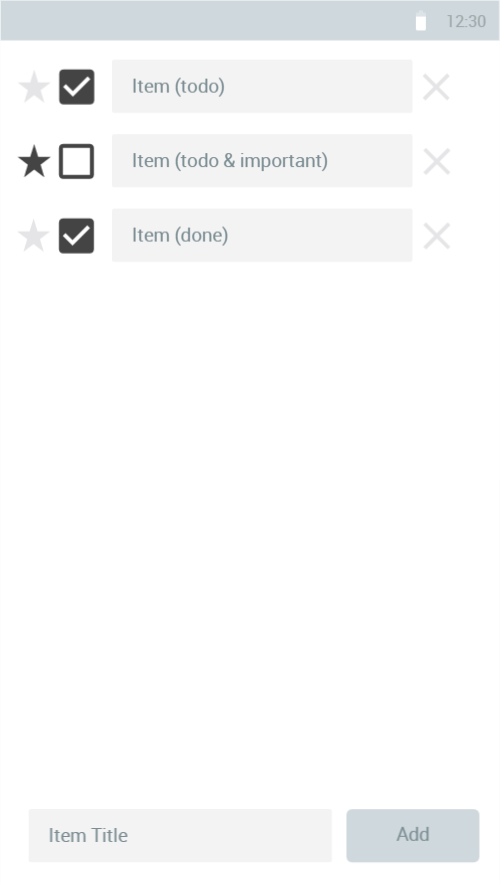
\includegraphics[scale=0.5]{img/fig/4-3-1_wireframe.png}
	\centering
	\caption{Wireframe der App}
	\label{fig:wireframe}
\end{figure}

Eine Besonderheit in der Darstellung lässt sich innerhalb der priorisierten Elemente finden. Um diese weiter hervorzuheben, werden diese an den Anfang der Liste gesetzt. Es entstehen somit zwei Teillisten, welche sich jedoch in derselben Listenansicht befinden. Wird nun ein zuvor nicht-priorisierter Eintrag priorisiert, so wechselt dieser seine Position ans Ende der Liste mit den bereits priorisierten Einträgen (bzw. wird oberhalb der ersten nicht-priorisierten Elements platziert). Alle Einträge zwischen der alten und der neuen Position des gerade betrachteten Eintrags werden um eine Listenposition nach unten verschoben. Bei Entfernen der Priorisierung wird das entsprechende Element nun nicht an seine ursprüngliche Position vor der Priorisierung, sondern an den Anfang der nicht-priorisierten Liste verschoben. Entfernt man also bspw. die Priorisierung des letzten Elements in der priorisierten Liste, ändert sich die Reihenfolge nicht. Dieses Verhalten kann vereinfacht in der untenstehenden Abbildung dargestellt werden.

Grundsätzlich werden alle Einträge in der Reihenfolge dargestellt, wie sie angelegt wurden, mit den eben beschriebenen Ausnahmen.

Um ebenfalls für farbliche Konsistenz zu sorgen, werden die beschriebenen Elemente auf Basis der folgenden Tabelle in ihrem Erscheinungsbild konfiguriert:

\begin{table}[h!]
	\centering
	\begin{tabular}{ |c|c|c|}
		\hline
		\textbf{Bezeichnung} & \textbf{Hex-Code} & \textbf{Darstellung}\\
		\hline
		
		
		\hline
		\multicolumn{3}{|c|}{\textbf{Allgemeines}}\\
		\hline
		Hintergrund & \texttt{\#F2F2F2} &\cellcolor[HTML]{F2F2F2}\\
		\hline
		Schriftfarbe & \texttt{\#8C8C8C} &\cellcolor[HTML]{8C8C8C}\\
		\hline
		
		
		\hline
		\multicolumn{3}{|c|}{\textbf{Bedienelemente}}\\
		\hline
		Hintergrund für inaktive Bedienelemente & \texttt{\#CECECE} &\cellcolor[HTML]{CECECE}\\
		\hline
		Hintergrund der Checkbox (angewählt) & \texttt{\#1A66FF} &\cellcolor[HTML]{1A66FF}\\
		\hline
		Schriftfarbe der Checkbox (angewählt) & \texttt{\#FFFFFF} &\cellcolor[HTML]{FFFFFF}\\
		\hline
	\end{tabular}
	\caption{Farbtabelle} \label{tab:farbtabelle}
\end{table}


\section{Nutzungszyklus} \label{sec:3-nutzungszyklus}
Der Nutzer öffnet die Anwendung. Beim Laden der Ansicht wird eine Datenbank-Funktion ausgeführt, um bereits existierende Einträge zu laden und ihre entsprechenden Beschreibungen samt weiteren Attributen in die einzelnen Zellen der Listenansicht zu laden. 

Der Nutzer möchte einen neuen To-Do-Eintrag erstellen. Dafür wird ein beschreibender Text in das Texteingabefeld am unteren Rand der Ansicht geschrieben. Um einen neuen Eintrag zu erstellen, wird ein beschreibender Text in das Texteingabefeld am unteren Rand der Ansicht geschrieben. Mit der Bestätigung über den \texttt{+}-Button wird ein neuer Eintrag in die Datenbank aufgefordert, wobei das \texttt{text}-Attribut mit dem zuvor gewählten Text aus dem Eingabefeld gefüllt wird. Die Zeichenfolge der \texttt{id} wird automatisch und zufallsbasiert generiert, \texttt{done} sowie \texttt{priority} standardmäßig auf \texttt{false} gesetzt. Der neue Eintrag wird unter den bereits vorhandenen Einträgen angefügt. Stern- sowie Häkchen-Symbol werden lediglich über ihre Kontur kenntlich gemacht.

Der Nutzer möchte den Test eines Eintrages ändern. Durch direktes Tippen auf den dargestellten Text in einer Zelle wird dies ermöglicht. Es erscheint ein Cursor, welcher ebenfalls Tastatur- und Berührgesten innerhalb dieses Feldes ermöglicht. Nach bestätigter Änderung über das Verlassen des Textfeldes (d.\ h. dem Tippen auf eine andere Stelle innerhalb der Ansicht) wird erneut eine Datenbank-Funktion ausgeführt. Diese bekommt das \texttt{ToDo}-Objekt übergeben und ersetzt den bestehenden Inhalt des \texttt{text}-Attributes mit dem nun geänderten.

Der Nutzer möchte den zuvor erstellten Eintrag priorisieren. Tippt dieser auf das Stern-Symbol, wird dieses mit der zuvor definierten Farbe gefüllt. Gleichzeitig bewegt sich das priorisierte Element an das Ende der Teilliste mit priorisierten Einträgen. Eine Datenbank-Funktion wird aufgerufen, welche den \texttt{priority}-Wert des übergebenen Objekts von \texttt{false} auf \texttt{true} setzt.

Der Nutzer möchte den zuvor priorisierten Eintrag als abgeschlossen markieren. Tippt dieser auf das Häkchen-Symbol wird dieses mit der zuvor definierten Farbe gefüllt. Eine Datenbank-Funktion wird aufgerufen, welche den \texttt{done}-Wert des übergebenen Objekts von \texttt{false} auf \texttt{true} setzt.

Der Nutzer möchte den zuvor als abgeschlossenen Eintrag aus der Liste der priorisierten Einträge entfernen. Tippt dieser auf das Stern-Symbol, wird dessen Füllung entfernt. Gleichzeitig bewegt sich das Element an den Anfang der Teilliste mit nicht-priorisierten Einträgen. Die zuvor ausgeführte Datenbank-Funktion wird erneut aufgerufen, welche den \texttt{priority}-Wert des übergebenen Objekts von \texttt{true} nun wieder auf \texttt{false} setzt.

Der Nutzer möchte den Eintrag abschließend entfernen. Tipps dieser auf das Kreuz-Symbol, wird der Eintrag aus der Liste entfernt. Die Elemente unterhalb des gelöschten Eintrags verschieben sich um jeweils eine Position nach oben. Eine Datenbank-Funktion wird aufgerufen, welche das übergebene Objekt des Eintrages aus der Datenbank entfernt.

		
	\chapter{Implementierung}
		\label{chap:implementierung}
		
	\chapter{Evaluation}
		\label{chap:evaluation}
		
	\chapter{Reflexion}
		\label{chap:reflexion}

%===========================================================================
%	BACK MATTER
%===========================================================================

	\pagestyle{plain}
	\clearpage
	\pagenumbering{alph}
	\printbibliography

\end{document}